\chapter{UPPAAL model}\label{ch:uppaalmodel}
For our models we use UPPAAL, an integrated tool environment used for modelling, simulating and verifying real time systems. When a model has been constructed, the model checker may be used to query invariant and reachability properties of the model. We choose UPPAAL, as we have previous experience with it, as well as the theory of timed automatas. In addition, many of its developers are located in Aalborg University along with the project group. Thus there is easy access to technical advice.

After a FESTO factory has been modelled, we may query it about its properties. The most interesting property is one of reachability; is it possible to reach a state, where x amount of products have been produced? If this is the case, UPPAAL may produce a shortest timed trace of actions needed to reach this state. However, the fastest trace is not always the best, for instance, a very fast trace may have the factory use up a lot of power. Thus, high throughput is not the only desired property for the factory, but a low cost is wanted as well. In order to involve costs, a branch of UPPAAL, called UPPAAL CORA\cite{UPPAALCORA} is used.

This program is very similar to regular UPPAAL, but it also allows for a global cost variable to be used, alongside the global clock. This variable is strictly non-decreasing. The cost can be increased either when an action is taken, or as a function of time, when waiting in a location. The model checker may explore the state space in a UPPAAL CORA model in a best-first manner. That is, it looks for a trace to the goal state with the smallest global cost value.

As mentioned in \cref{ch:introduction}, this project differs from others before it, as we are working with a system of not only one, but many different configurations. Thus, when modelling in UPPAAL CORA, a strong focus was put on not hard coding the model. Instead we design and implement templates, which can later be instantiated with different parameters. The instantiated templates can then be run in parallel, as a single functioning factory configuration.

In \cref{subs:recipe,subs:module,subs:remover,subs:coster}, the developed templates, that make up the current model, are explained.

\section{Recipe}
\label{subs:recipe}

\begin{figure}[h]
\centering
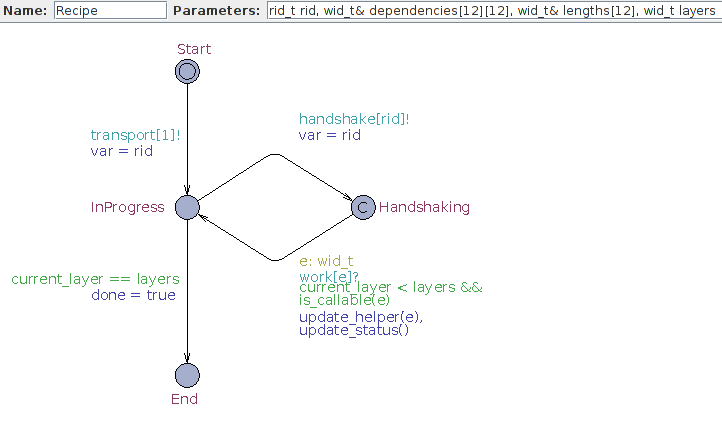
\includegraphics[width=\textwidth]{firstrecipe.png}
\caption{The model of the recipe template}
\label{fig:firstrecipe}
\end{figure}

To represent an item passing through a FESTO factory, the \emph{recipe template} is designed and implemented. This defines a set of steps that must be taken to create a specific product. A recipe synchronises with a module to have work performed on it. Each module has a specific type of work, which it may perform on a recipe. The \emph{recipe template} can be seen in \cref{fig:firstrecipe}.


A recipe is initialised with an ID, along with an array of arrays. The latter construct describes the dependency between steps, that must be taken for a recipe to move to its end location. Each array layer describes a set of steps that may be taken in an arbitrary manner. However all these steps must be taken, before any of the steps in the next layer may be taken. For instance, the dependency structure [[Hammer, Screw][Package]], means that the given recipe should get hammered and screwed before it is packaged. However the hammering and screwing may occur in an arbitrary sequence.


When transitioning from the \emph{start} location, a recipe will, through the \emph{transport} channel, synchronise with the first module in the production line. Through the global \emph{var} variable, the ID of the recipe is passed to the module in order for it to lay claim on it. This is part of a simple mutual exclusion scheme, making sure that a module can only work on one specific recipe at a time. Once a recipe is in progress, it may handshake with a module by using its ID to identify itself. When identified, the module may perform a work action upon the recipe to complete a pending recipe step. If a work action has been done, we make sure to mark the finished step as done, so that it is not repeated. In the case that all steps have been taken, in a layer of the dependency array, we make sure to move onto the next. Once all layers have been completed, we may pass to the end location. Here, we set the local \emph{done} variable to true. This is used to query our model checker to see if we can reach a state where the recipe is finished. For a recipe, \emph{r1}, the query would be: \[E<> r1.done\]

\section{Module}
\label{subs:module}

\begin{figure}[h]
\centering
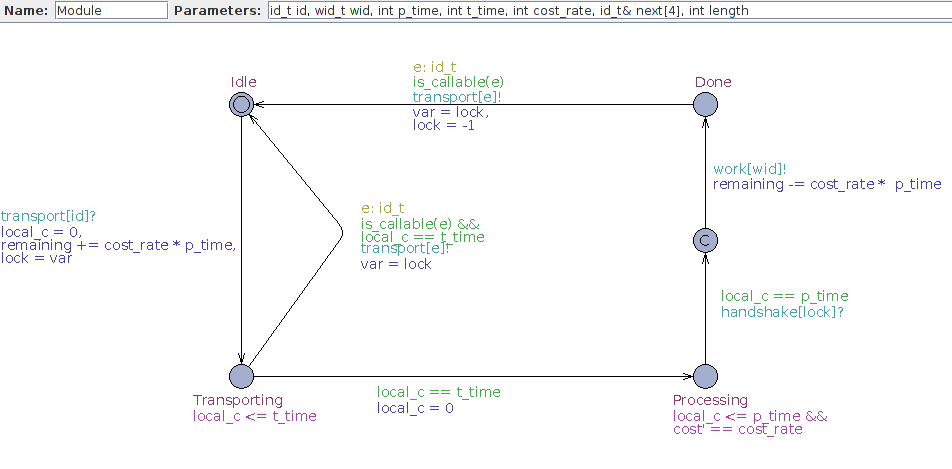
\includegraphics[width=\textwidth]{firstmodule.png}
\caption{The model of the module template}
\label{fig:firstmodule}
\end{figure}

The \emph{module template} models a module in a FESTO factory. A module is identified by its ID parameter. A second parameter \emph{wid} (work id) indicates the type of work the module may perform on a recipe. A module also includes an array, \emph{next}, which contains IDs of modules, which it may pass an item onto. The \emph{module template} can be seen in \cref{fig:firstmodule}.


To transition from the \emph{idle location}, a module must receive an item from a module earlier in line by synchronising on the \emph{transport} channel.
As stated in \cref{subs:module}, the first \emph{transport} occurs between a recipe and the first module in line. This also passes the recipe ID onto the module, in order to lock other recipes out, saving the recipe ID in the \emph{lock} variable. From this point on, when a module synchronises on \emph{transport}, it passes the recipe ID onto the next module for locking.

After transitioning to the \emph{transporting} location, the module waits for \emph{t\_time}. Afterwards it may synchronise on \emph{transport} again, to send the recipe to one of the next modules in line. Instead of passing on the recipe, we may try to work upon it.

By giving the option of working or passing through, we simulate that some items do not need to be worked on, by every module in the production line. If we decide to work on the recipe, we go to the \emph{processing} location and wait for \emph{p\_time}. Each time we delay by a single time unit in this location, the global \emph{cost} variable is increased by the value of \emph{cost\_rate}. Once \emph{p\_time} has passed, the module can identify its recipe through a handshake by using the recipe ID saved in \emph{lock}. Once it is confirmed, that the module is working with the correct recipe, it will synchronise on the \emph{work channel}, finishing its job upon the item. Once finished, the module may go back to the \emph{idle} location by transporting the item to one of the next modules in line.

\section{Remover}
\label{subs:remover}

\begin{figure}[h]
\centering
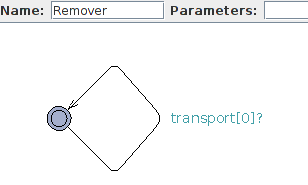
\includegraphics[width=0.6\textwidth]{firstremover.png}
\caption{The model of the remover template}
\label{fig:firstremover}
\end{figure}

The \emph{remover template} is not very complex, and can be seen in \cref{fig:firstremover}. It continously tries to synchronise on the \emph{transport} channel 0, in order to remove a recipe from the factory. The factory modules each have their own \emph{transport} channel, given by their ID, which is 1-indexed. Thus, a \emph{transport} on channel 0 does not pass the recipe to a module, but instead to the remover. If we want to remove a recipe, when it is passed on from a specific module, we simply set one of the IDs in the module’s next array to 0. Removing a recipe from a factory is especially beneficial in circular setups, as a finished recipe may otherwise be passed around indefinitely. This may unnecessarily decrease factory throughput. By removing recipes. We also decrease the state space that needs to be searched by the model checker.

\section{Coster}
\label{subs:coster}

\begin{figure}[h]
\centering
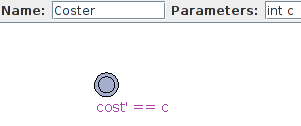
\includegraphics[width=0.6\textwidth]{firstcoster.png}
\caption{The model of the coster template}
\label{fig:firstcoster}
\end{figure}

The \emph{coster template} ensures that parallel processing of recipes is prefered, during a best-first Search. It can be seen in \cref{fig:firstcoster} The \emph{coster template} is initialised with a rate \emph{c}, which increases the \emph{cost} variable as a function of the global time passed. Without this, the search would not have any reason to run several modules at the same time as the final \emph{cost} would not change. By having a constant \emph{cost} on the factory’s operating time, we make the prospect of parallel processing a prefered option.

%\section{Running UPPAAL CORA through Python}
%Having defined our model, we can now use UPPAAL to instantiate a specific factory configuration and generate a best cost trace. However, we are are interested in comparing several configurations and from those pick the one with the best performance. Manually instantiating each configuration and developing a trace would be very time consuming. Instead, we work with our UPPAAL CORA models in a programmatic manner. This way we may write scripts for generating configurations and for each of these configurations, we can use UPPAAL CORA to generate a trace. Through the script we can then use the generated traces to pick the best configuration.

%We choose to script in Python 3.5 as it very simple to work with and the majority of group members have some experience with it. Python is not known for its fast computation, but most of the execution load will lay upon UPPAAL CORA, so this is not a great concern. 


%Out of the box, UPPAAL CORA does not have an API, so that we may interact with it through Python. The actual model checker part of the UPPAAL CORA installation lies in the verifyta executable. This may be called through the terminal. It takes two arguments, an XML file describing the given configuration and a file containing property queries. Additional arguments may involve the type of search, what kind of trace to generate etc. After run, results are written to the terminal. 


%In order to model check a configuration using python, we must create both an XML and a query file. The query file is simple as it needs only one query that checks whether it is possible for all recipes to end up in the “done” state. The XML file is a bit more difficult to handle. UPPAAL saves all information about a given project in an XML file. This Includes templates, global variables and the system declaration. In our case we have a project that includes the templates as described in \cref{sec:DesignAndImplementationInUPPAALCORA}. We may now edit this XML file, so that it creates the configurations we want to do model checking on.

%Based on a specific optimization problem the global declaration and system declaration need to be edited. In the global declaration, we must edit the amount of modules, worktypes and recipies present for the problem. These amounts are used to declare the correct channels and user defined types. In the system declaration, we must instantiate the recipes that need to be worked on, as well as a single instance of both the remover and the coster. For each specific factory configuration we then edit the system declaration further, by instantiating modules and connecting them according to the configuration specified. 


%A python script that handles a specific optimization problem should do the following. Take a set of recipes as input along with a set of modules. Generate a query file based on the number of recipies. Set up a base XML file according to the problem. Use the base to generate an XML file for each candidate, which may solve the problem. Each candidate should use only the modules specified in input. For each of the candidate XML files, run it on the verifyta executable along with the query file, making sure to set the options for generating the best cost trace. After each individual run, the script can extract the cost of the trace from the terminal output. Once all configurations have been run through we can compare the results. The configuration generating the lowest cost trace is picked as the solution. 


%With this overall execution plan we set up some complex questions which need to be answered. The pool of potential candidates is very large for any real problem, so a linear search is not very efficient. We need to restrict both what kind of candidate configurations we want to consider, in order to limit the search space. In addition we must find an efficient way to search through candidates. These questions will be tackled in the last two sections of this chapter. 
